\label{sec:beyond}
In practice, usefulness of an access control system depends on many other aspects beyond its expressive power. For example, in the NIST special publication \textit{Guidelines  for Access Control System Evaluation Metrics} \cite{access-control-evaluation}, the authors divide these aspects into four categories including (i) administration, (ii) enforcement, (iii) performance and (iv) support. In this section, we mostly focus on administrative properties. We compare the aforementioned models from two perspectives - single attribute vs multi-attribute and enumerated vs logical-formula authorization policy.

\subsection{Single attribute vs multiple attributes}

We have seen earlier that \EPOneOneModels{} is equivalent to \EPMNModel{} and \LPOneOne{} is equivalent to \LPMN{}. But, in practice this may not be useful because of many reasons including the following.

\textbf{Attribute-value assignments and administration.} Ranges of each attribute intrinsically separate their values. For example, if \textit{role} and \textit{location} are two different attributes, values of these attributes are inherently distinguished. As a result, attribute-value assignments to users and objects and administration of these values (add or remove existing values) can be separated using semantics of individual attributes.

\textbf{Privacy concern.} If we combine values of  more than one attributes into single attribute values, a user may expose more credential than required in a particular context.  For example, combining values \textit{role} and \textit{location}, we may create values \{\textit{manager@campus, manager@home}\}. If so, a user cannot hide role  when the context requires only his location.



 \newcommand{\highlight}[1]{%
 	\colorbox{black!19}{$\displaystyle#1$}}
 
\begin{table}
	\centering
	\caption{ Different representations of  $Auth_{read}$ policy  ($Auth_{read}$ states that \textit{\manager} can access \textit{TS} objects being from either \textit{office} or \textit{home})} 
	\label{tab:LAP-heterogeneity}
	\begin{tabular}{|l|}						
		\hline					
			
			(i) $  \manager \in role(u) \land (office \in location(u) \highlight {\lor home \in location(u)})  \land TS \in sensitivity(o)$ \\
			(ii) $((\manager \in role(u) \land office \in location(u) ) \highlight {\lor (\manager \in role(u) \land home \in location(u) )}  )$ \\ \hfill $ \land TS \in sensitivity(o)$\\
			(iii) $((\manager \in role(u) \land office \mathbf{\in}\in location(u) \land TS \in sensitivity(o) ) \highlight{\lor}$  \\ \hfill $\highlight{((\manager \in role(u) \land home \in location(u) \land TS \in sensitivity(o) )}$ \\
		 \hline	
	\end{tabular}	

	
\end{table}


\textbf{Larger set to manage.} Combining values of more than one attribute together, we often need to manage larger set of values. For example, if there are ten possible values of \textit{role} and ten possible values of \textit{location}, by combining them we may need to manage one hundred values.  



\subsection{Enumerated vs logical-formula authorization policy}
In this section, we consider pros and cons of logical-formula and enumerated   authorization policy. Usually, logical formula   allows us powerful language construct to formulate even complicated business logic and policies in a succinct way. Logical formulas often support large number of logical and relational operators which make it easy to set up new policies. On the downside,  logical formulas impose little constraint on the structure, size or style of the authorization policy. As a result, policies are heterogeneous in nature having different sizes and styles. Even a single policy can be represented in so many ways.  For example, Table \ref{tab:LAP-heterogeneity} shows how a policy $Auth_{read}$ can  be represented in different three forms. The heterogeneity across multiple policies and lack of a canonical form make it difficult to understand, update or administer existing policies.  For example, to update $Auth_{read}$ so that \textit{manager} no longer gets access from \textit{home}, different representations of the policy need to be updated in different ways. Required changes to policies are highlighted in Table \ref{tab:LAP-heterogeneity}. These changes require  manual effort  by an administrator to update them. In a different aspect, LAPs are often monolithic, making it difficult to distinguish sub-policies.




On the other hand, enumerated authorization policies (EAPs), have a distinct form of representation. Thus, in \EPModels{} models, policies are homogeneous and  sub policies in a policy can be presented in one or more tuples and a  policy is a set of such tuples. Different tuples are distinguishable from each other and can be thought of as micro-policies. Thus, policies in enumerated tuples are polylithic as opposed to monolithic in logical formula. 

%Usefulness of micro policies is further discussed in Section \ref{sec:usefulness}.

On the flip side, an EAP can be very large as it  does not allow conditional expressions. For example, the  condition \textit{$age(u) \ge 18$}, should be achieved by enumerating all possible ages greater or equal 18. Another disadvantage  is that when we add/remove attributes from the system, existing EAPs may require to be updated. 

\vspace{-1em}

\subsubsection{Administration using micro-policies}
\label{sec:usefulness}

The policy $Auth_{read}$ mentioned above can be represented using micro-policies as $\{( \{\manager\}, \{office\}, \{TS\} )$, $( \{\manager\}, \{home\}, \{TS\} )\}$. In order to update the policy so that \textit{manager} can no longer access from \textit{home}, we can remove the second tuple resulting $Auth_{read} \equiv \{( \{\manager\}, \{office\}, \{TS\} )\}$. Similarly, we can add new micro-policies adding new tuples to $Auth_{read}$.

Thus, in term of administration, the minimum administrative units in EAP are micro-policies represented by policy tuples. So, it is possible that an EAP can be managed by multiple administrators at the most fine grained level of micro-policies. Design of an administrative model to manage micro-policies is beyond the scope of this paper. We postulate that as policy update can be done by merely adding or removing policy tuples,  it can be done programmatically  in \EPModels{} model. Figure \ref{fig:policy-pros-cons} shows pros and cons of \EPModels{} and \LPModels{} models. Table \ref{tab:pros-cons-table} presents a detailed comparison.




\vspace{-1em}


\subsubsection{Canonicalization of enumerated authorization policy}

In this section, we show how we can represent EAPs in a canonical form. Consider, $Auth_{write} \equiv \{( \{\manager\}, \{TS\} )$, $ ( \{\manager, dir\}, \{TS\} )\}$ in $EP$-$ABAC_{1,1}$. The first tuple says someone who is at least manager (can additionally have any other roles) can write \textit{TS} objects. The second tuple says someone both manager \& director (may additionally have any other roles) can write \textit{TS} objects. Thus, the first tuple also includes authorization requirements of the second tuple. So, if we update $Auth_{write}$ to remove the second tuple,  effectively updated $Auth'_{write}$ also represents the old policy. Thus, an enumerated authorization  policy can be represented in more than one ways which violates uniqueness of the canonical form. The advantage of representing policies in canonical form is that we make sure by adding or removing tuples, we really update the policy.  This would help  in the automation of policy administration. 


% It authorizes a \textit{manager } to access \textit{TS} objects from  \textit{office}. If the same \textit{manager} additionally holds a \textit{director} role, $Auth_{read}$ also authorizes him. This is because the authorization function checks if the requester at least (not exactly) possesses the values specified in the tuple.  Thus, if  we update $Auth_{read}$ to add a new tuple $(\{manager, director\}, \{office\}, \{TS\})$, the updated policy semantically represents the same old policy. (because the new tuple is subsumed by another tuple in the policy). Thus, an EAP can be represented in more than one forms which violets uniqueness of canonical form. 


 	\begin{figure} 
 		\centering
 		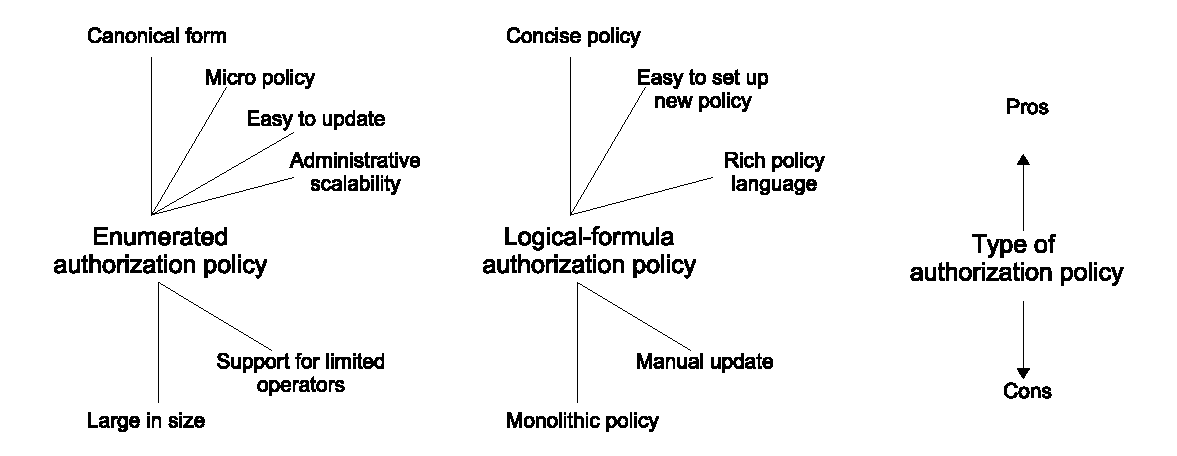
\includegraphics[width=.9\textwidth]{DBSEC16/policy-pros-cons}
 		\caption{Pros and cons of enumerated and logical-formula authorization policy}
 		\label{fig:policy-pros-cons}
 	\end{figure}

\begin{table}[]
\centering
\caption{Comparison of  LAP  and  EAP }
\label{tab:pros-cons-table}
\begin{tabular}{|c|c|c|}
	\hline
Characteristics    of   &  \begin{tabular}[c]{@{}l@{}} LAPs  (considering \\ $ABAC_\alpha$/HGABAC)  \end{tabular}     & \begin{tabular}[c]{@{}l@{}}  EAPs  (value enumeration \\ for  positive attribute-values) \end{tabular}        \\ \hline
\multicolumn{3}{l}{} \\ 
\multicolumn{3}{l}{\textit{\textbf{Definition}}} \\ \hline
\begin{tabular}[c]{@{}l@{}} \textit{distinguishing features}\end{tabular} & \begin{tabular}[c]{@{}l@{}}  logical-formula \end{tabular} & \begin{tabular}[c]{@{}l@{}}  enumeration\end{tabular} \\ \hline
\multicolumn{3}{l}{} \\ 
\multicolumn{3}{l}{\textit{\textbf{Syntax}}} \\ \hline

\begin{tabular}[c]{@{}l@{}}\textit{Representation} \end{tabular} & \begin{tabular}[c]{@{}l@{}} expression \end{tabular} & \begin{tabular}[c]{@{}l@{}} set  \end{tabular} \\ \hline

\begin{tabular}[c]{@{}l@{}}\textit{Morphism} \end{tabular} & \begin{tabular}[c]{@{}l@{}} polymorphic (single policy can \\  be represented many ways) \end{tabular} & \begin{tabular}[c]{@{}l@{}} unique representation \end{tabular} \\ \hline

\begin{tabular}[c]{@{}l@{}}\textit{Policy type}\end{tabular} & \begin{tabular}[c]{@{}l@{}} macro-policy, \\ possibly cohesive sub-policies\end{tabular} & \begin{tabular}[c]{@{}l@{}} micro-policy, \\ disjointed sub-policies  \end{tabular} \\ \hline

\begin{tabular}[c]{@{}l@{}}\textit{Divisibility}\end{tabular} & \begin{tabular}[c]{@{}l@{}} monolithic\end{tabular} & \begin{tabular}[c]{@{}l@{}} polylithic  \end{tabular} \\ \hline


\begin{tabular}[c]{@{}l@{}}\textit{Size}\end{tabular} & \begin{tabular}[c]{@{}l@{}} usually concise\end{tabular} & \begin{tabular}[c]{@{}l@{}}  usually large  \end{tabular} \\ \hline

\begin{tabular}[c]{@{}l@{}}\textit{Language}\end{tabular} & \begin{tabular}[c]{@{}l@{}} propositional/ \\ first-order logic formula\end{tabular} & \begin{tabular}[c]{@{}l@{}} equivalent to DNF \\  of logical formula  \end{tabular} \\ \hline

 
 \multicolumn{3}{l}{} \\ 
 \multicolumn{3}{l}{\textit{\textbf{Semantics}}} \\ \hline
 
 \begin{tabular}[l]{@{}l@{}}\textit{Set of granted  privileges} \end{tabular} & \begin{tabular}[c]{@{}l@{}} dynamic (may change on addition/ \\removal  of attribute-values)\end{tabular} & \begin{tabular}[c]{@{}l@{}}static (privilege is explicitly\\ granted) \end{tabular} \\ \hline 


 \begin{tabular}[c]{@{}l@{}}\textit{Required attribute-value }\\ \textit{assgnments for granting} \\ \textit{privileges} \end{tabular} & \begin{tabular}[c]{@{}l@{}} partial assignments may \\  grant privilege\end{tabular} & \begin{tabular}[c]{@{}l@{}} requires complete assignment  \end{tabular} \\ \hline 
 
% \begin{tabular}[c]{@{}l@{}}\textit{ Privilege abstraction} \end{tabular} & \begin{tabular}[c]{@{}l@{}} may abstract granted privileges\end{tabular} & \begin{tabular}[c]{@{}l@{}} no privilege abstraction  \end{tabular} \\ \hline 

\multicolumn{3}{l}{} \\ 
\multicolumn{3}{l}{\textit{\textbf{Administration}}} \\ \hline

\begin{tabular}[c]{@{}l@{}}\textit{Cost of reviewing policy} \end{tabular} & \begin{tabular}[c]{@{}l@{}} NP-complete \end{tabular} & \begin{tabular}[c]{@{}l@{}} polynomial \\ (in number of tuples) \end{tabular} \\ \hline

%\multicolumn{3}{l}{\textit{\textbf{Privilege administration}}} \\ \hline

\begin{tabular}[c]{@{}l@{}}\textit{Granting new privilege} \end{tabular} & \begin{tabular}[c]{@{}l@{}} manual update \end{tabular} & \begin{tabular}[c]{@{}l@{}} add new tuples \end{tabular} \\ \hline

\begin{tabular}[c]{@{}l@{}}\textit{Remove existing privileges} \end{tabular} & \begin{tabular}[c]{@{}l@{}}manual update  \end{tabular} & \begin{tabular}[c]{@{}l@{}} remove tuples \end{tabular} \\ \hline 

\begin{tabular}[c]{@{}l@{}}\textit{Minimum administrative unit} \end{tabular} & \begin{tabular}[c]{@{}l@{}} entire policy \end{tabular} & \begin{tabular}[c]{@{}l@{}} micro-policy \end{tabular} \\ \hline   

\begin{tabular}[c]{@{}l@{}}\textit{scalability} \end{tabular} & \begin{tabular}[c]{@{}l@{}} not scalable  \end{tabular} & \begin{tabular}[c]{@{}l@{}} \hfil scalable \end{tabular} \\ \hline     

\multicolumn{3}{l}{} \\ 
\multicolumn{3}{l}{\textit{\textbf{Application}}} \\ \hline

\begin{tabular}[l]{@{}l@{}}\textit{} Convenient for \end{tabular} & \begin{tabular}[c]{@{}l@{}} specifying new policy, \\  administration using range \\ of attribute-values\end{tabular} & \begin{tabular}[c]{@{}l@{}}  updating policy, \\ fine grained administration\end{tabular} \\ \hline 

\begin{tabular}[l]{@{}l@{}}\textit{} Suitable environment \end{tabular} & \begin{tabular}[c]{@{}l@{}} open, loosely administered system, \\ distributed administration\end{tabular} & \begin{tabular}[c]{@{}l@{}}  close, tightly administered \\ system\end{tabular} \\ \hline 

                                        
\end{tabular}
\end{table}

To represent \EAP{}s in a canonical form, we ensure that in the same policy, no policy-tuple subsumes another policy-tuple. Formally, let $t_i$ denotes $i^{th}$ tuple in a policy and $S_{ik}$  be the $k^{th}$ set in tuple $t_i$. We say, a policy tuple $t_i$ subsumes $t_j$ iff  $(\exists p \in \{1,2,..,m+n\}, \forall q \in \{1,2,..,m+n\} \setminus {p})[S_{ip} \subseteq S_{jp} \land (S_{iq} \subseteq S_{jq} \lor S_{ip} = S_{jp}) ]$. For example, for $t1=(\{\manager,dir\}, \{TS\})$,$t2=(\{\manager, dir, adv\}, \{TS\})$, $t3=(\{\manager,dir, adv\}, \{H\})$ t1 includes t2 but none of t1 and t2 includes t3. 



To maintain a canonical representation of EAPs, we can remove policy-tuples that have been subsumed by other tuples. It is also possible to specify more sophisticated meta policies to manage subsumed policy-tuples.  



